%!TEX root = ../Thesis.tex
%\chapter{Long chapter title with $\pi$ $π$ or π}
%\chapter{Long chapter title with \texorpdfstring{$\pi$ $π$ or π}{π π or π}}
\section{Correlation of Fractures From Core, Borehole Images and Seismic Data in a Chalk Reservoir in the Danish North Sea}
\label{seg:talaEAGE}
\paragraph{Abstract:} We present an integrated fracture study in the Ekofisk chalk reservoir of the Kraka Field, offshore Denmark, based on core, borehole images and seismic data. The core contains numerous fractures ranging from short (cm-scale) fractures, mostly associated with chert or stylolites, to large (m-scale) open, slickensided fractures likely related to halokinesis. On borehole images, especially larger fractures are identified, coinciding in dip and dip-azimuth. Seismic data at an approximate resolution of 40m would not resolve these local features around the well-bore. We show that chromatic analysis combined with an ant-tracking algorithm extracts several lineaments (> m-scale) from the seismic data. These correlate closely in orientation and distribution with the fractures logged in the well data. It is likely that these represent fracture corridors, small faults or damage zones in the chalk. The seismic data therefore provides a valuable method for mapping the size, orientation and connectivity of fracture zones away from the well. This gives insights into the scalability of local stress fields, and fracture distributions. 

{\vfill\hfill\newline\fbox{\parbox{.97\textwidth}{\fullcite{aabo2017correlation}}}}

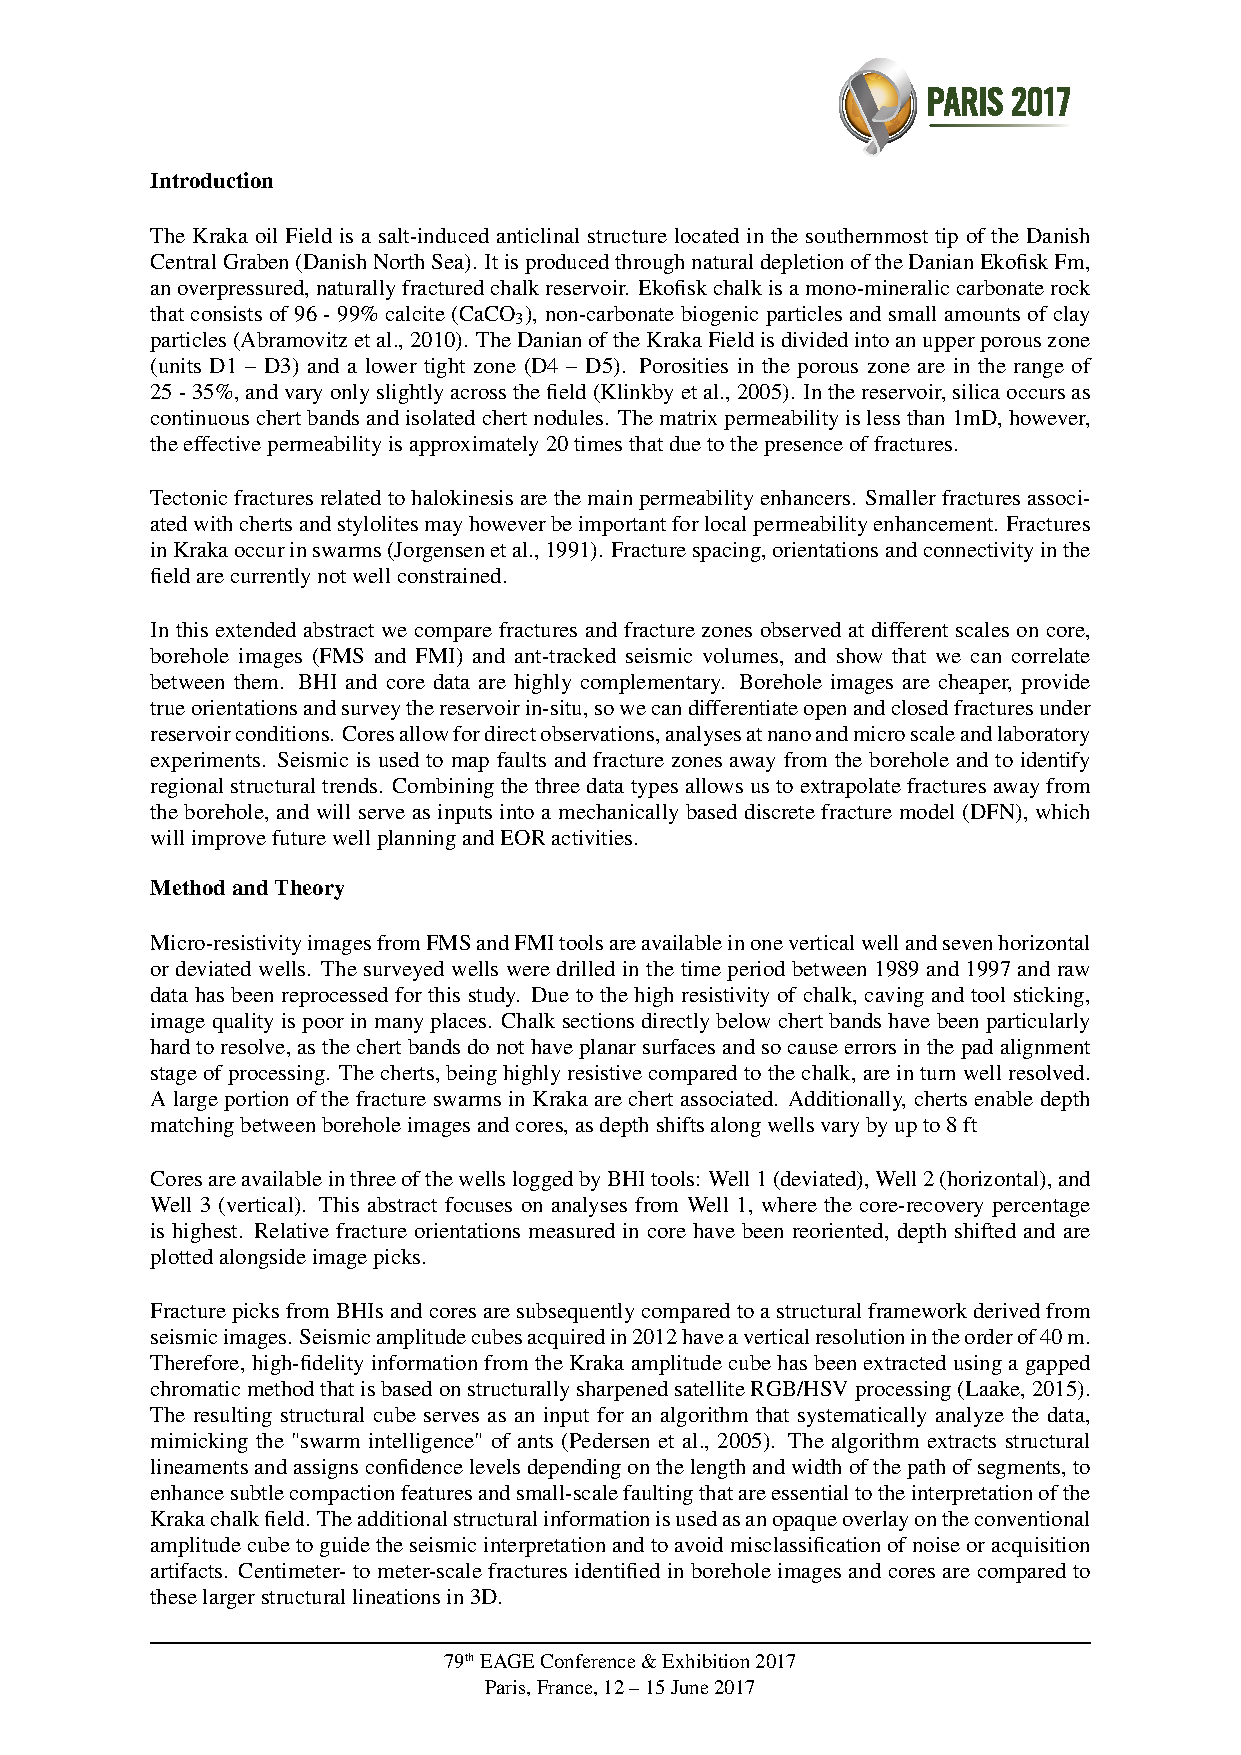
\includepdf[pages=1-4,pagecommand={},width=1.2\textwidth,offset=0.7cm -1.5cm]{papers/2017.1}

\todo{Fix Alignment}